\section{Trigger efficiencies}
\label{app:triggerEff}

In this section we collect all trigger efficiency maps as described in Sec.~\ref{sec:trigger}. 

\begin{figure}[h!]
  \centering
  \subfloat[][only 2l, low $|\eta|$]    {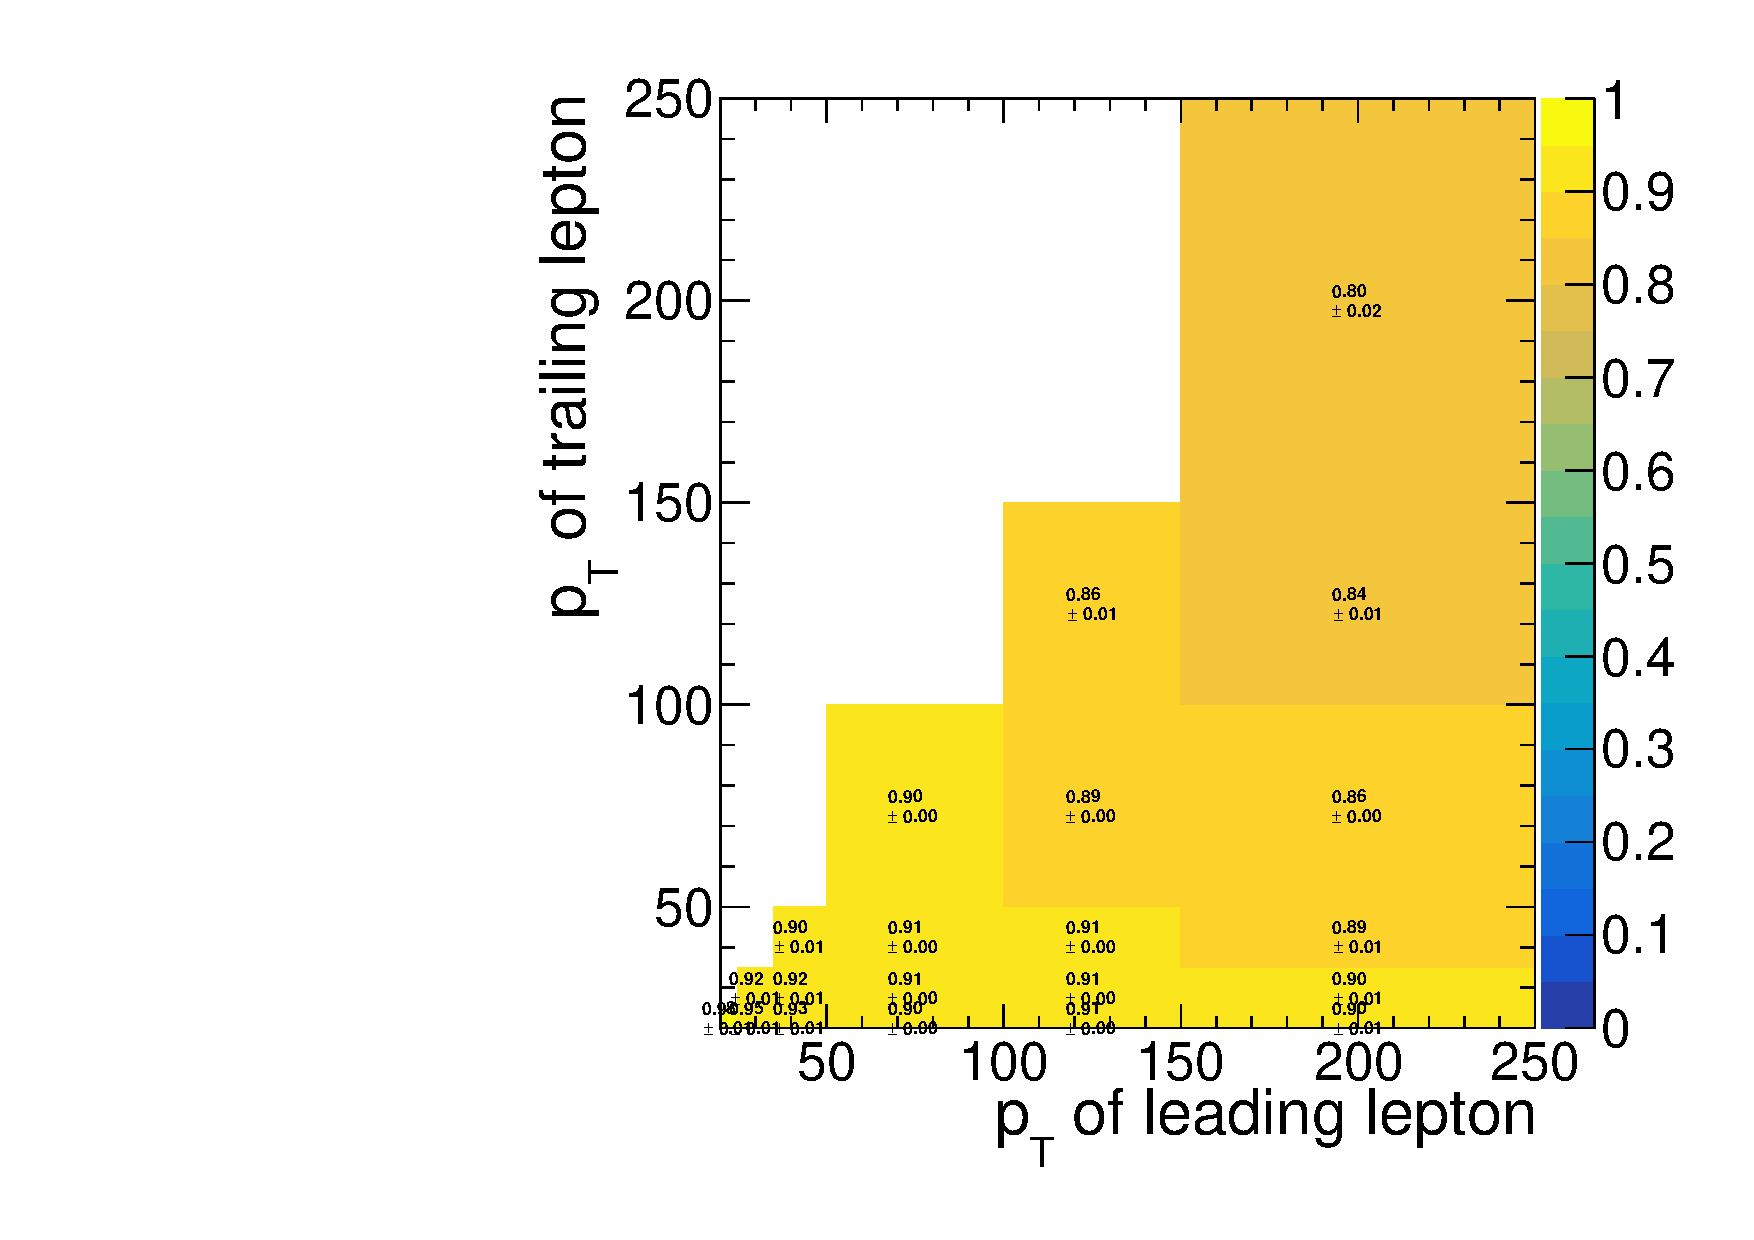
\includegraphics[width=0.45\textwidth]{figures/trigger/HLT_mumuIso_pt1_pt2_lowEta1_veryCoarse.pdf}}
  \subfloat[][2l+backup, low $|\eta|$]  {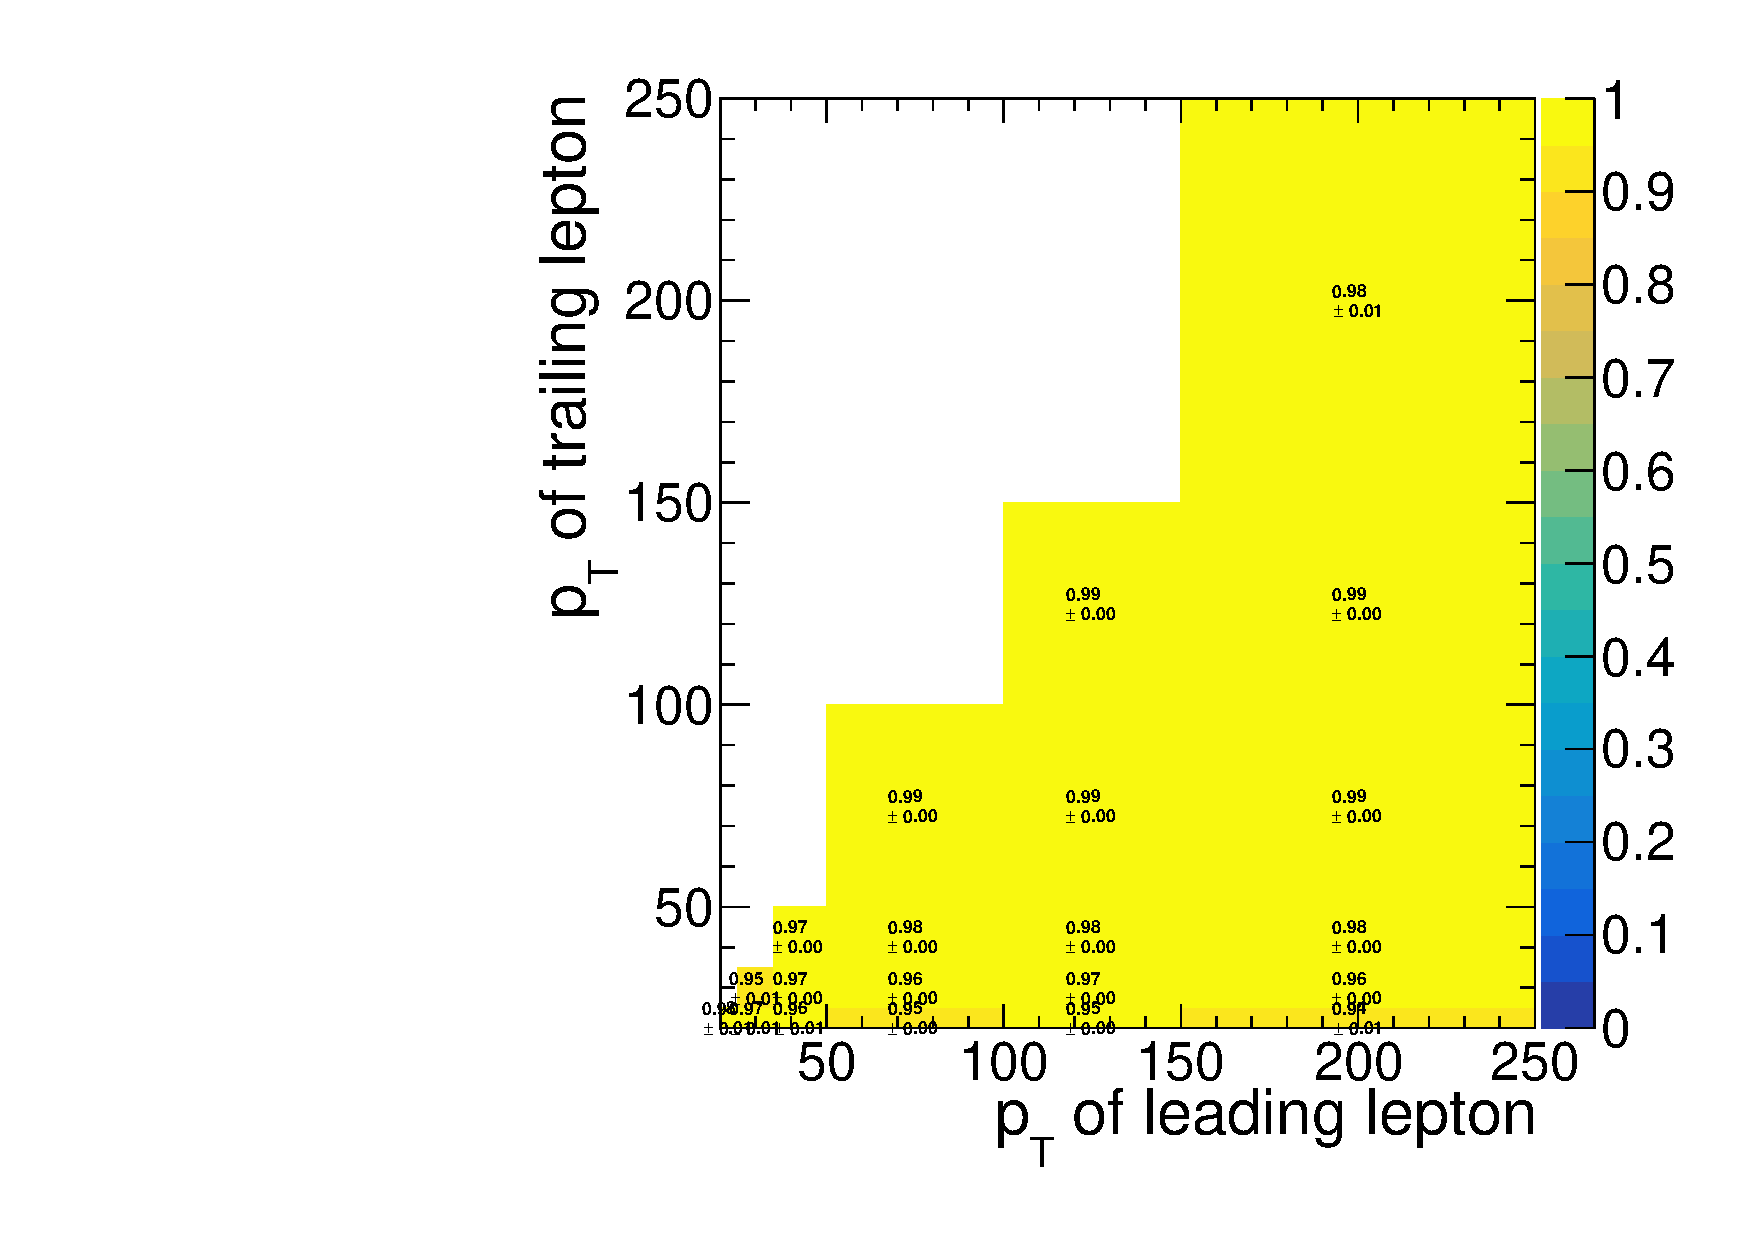
\includegraphics[width=0.45\textwidth]{figures/trigger/HLT_mumuIso_OR_HLT_mumuNoiso_OR_HLT_SingleMu_noniso_pt1_pt2_lowEta1_veryCoarse.pdf}}\\
  \subfloat[][only 2l, high $|\eta|$]   {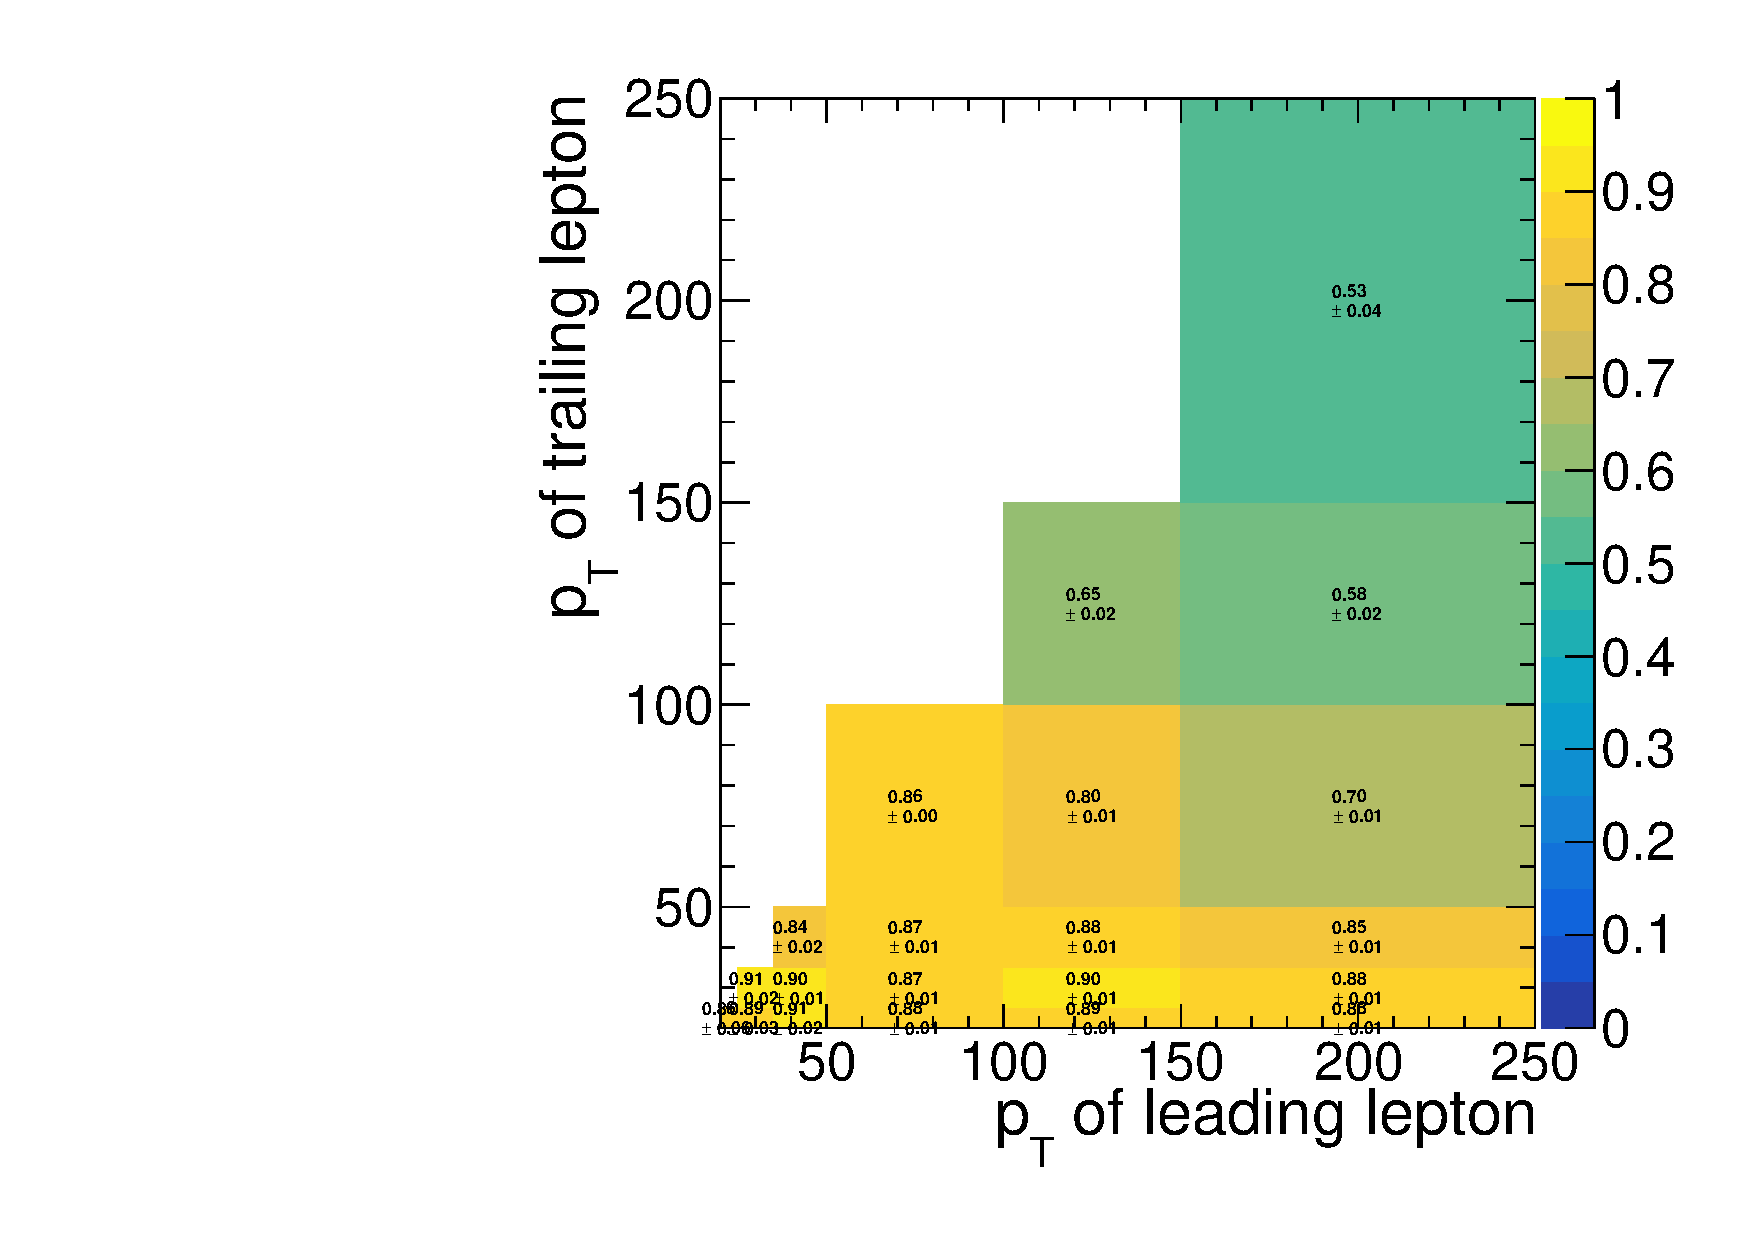
\includegraphics[width=0.45\textwidth]{figures/trigger/HLT_mumuIso_pt1_pt2_highEta1_veryCoarse.pdf}}
  \subfloat[][2l+backup, high $|\eta|$] {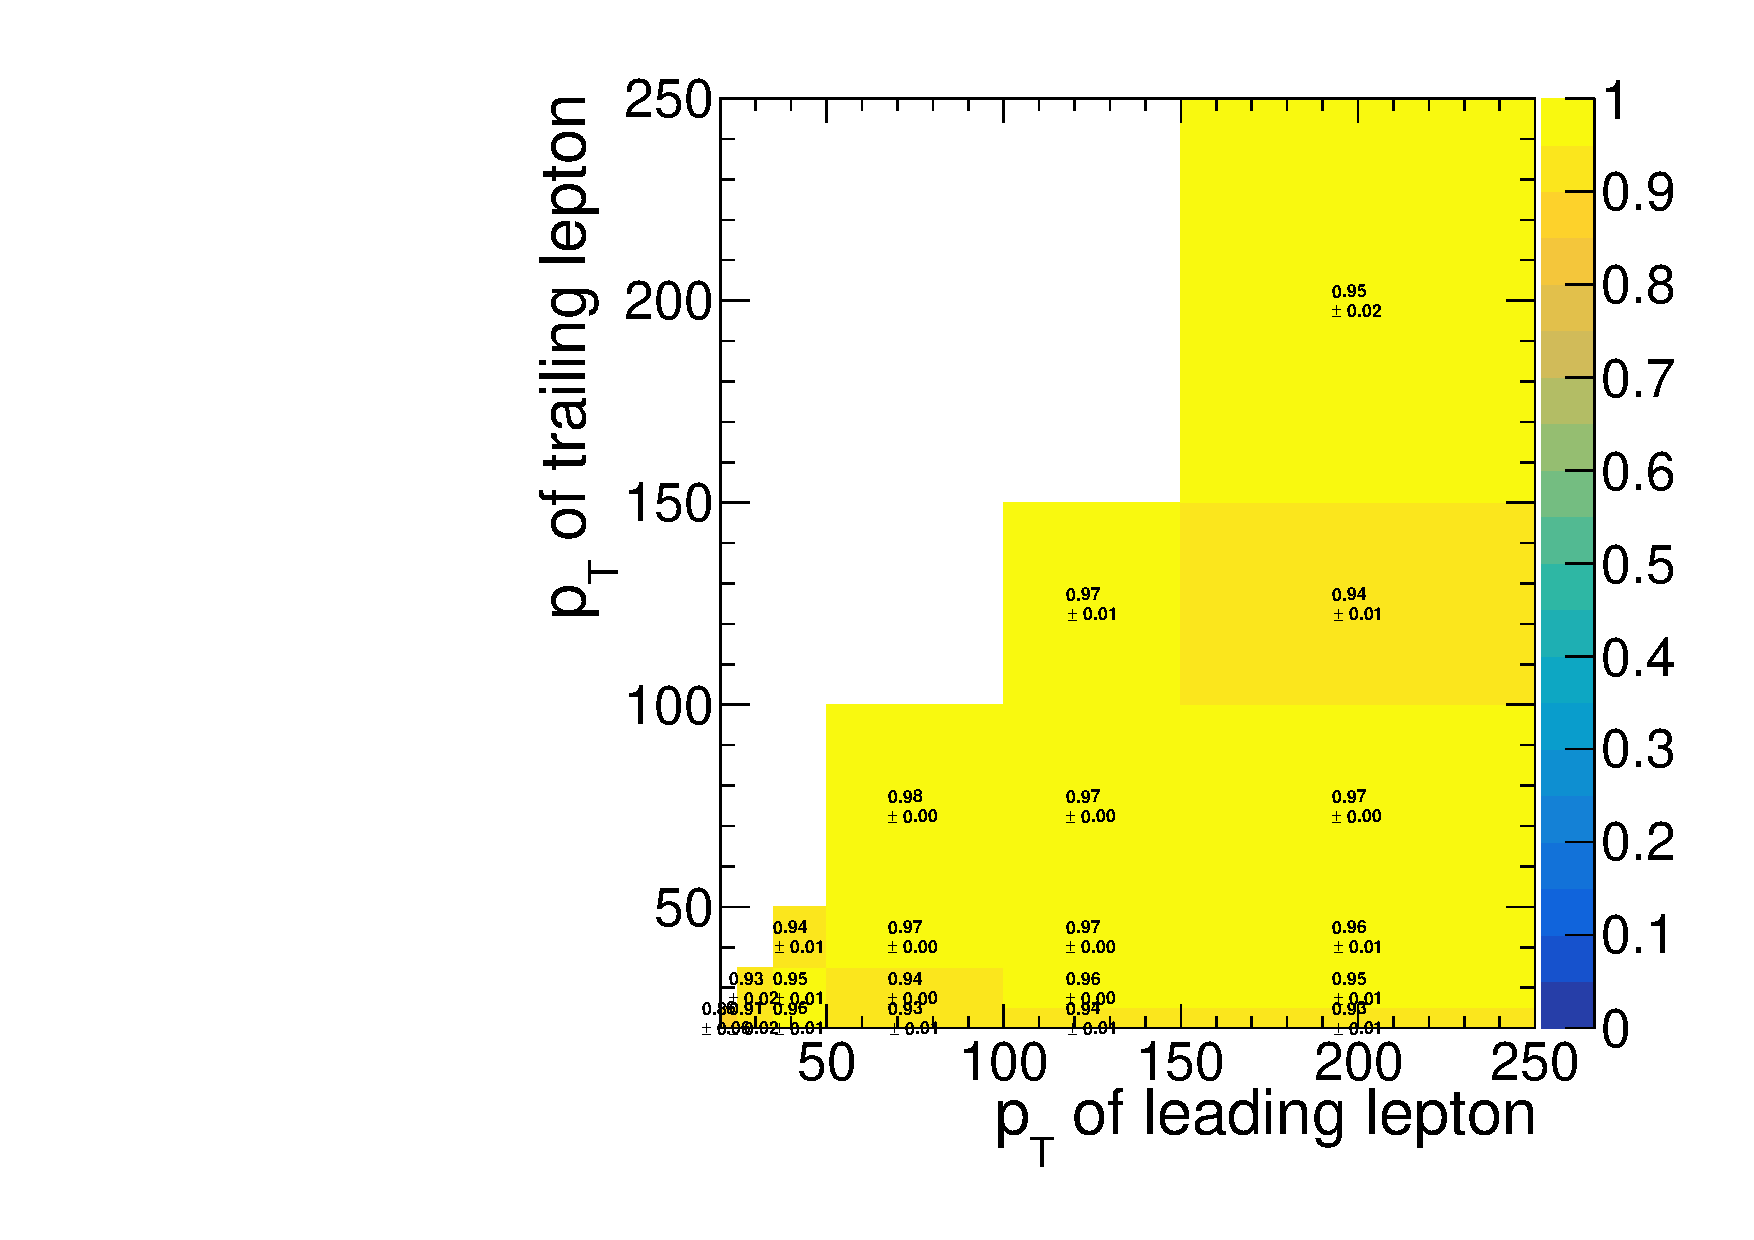
\includegraphics[width=0.45\textwidth]{figures/trigger/HLT_mumuIso_OR_HLT_mumuNoiso_OR_HLT_SingleMu_noniso_pt1_pt2_highEta1_veryCoarse.pdf}}
  \caption{Trigger efficiency maps for the e$\mu$ channel for $\eta$<1.5 (top) and $\eta>1.5$ (bottom) of the leading lepton. The plots on the left show the efficiency of the 
double lepton triggers without the single lepton backup.}
  \label{fig:mumu_triggerEff}
\end{figure}

\begin{figure}
  \centering
  \subfloat[][only 2l, low $|\eta|$]    {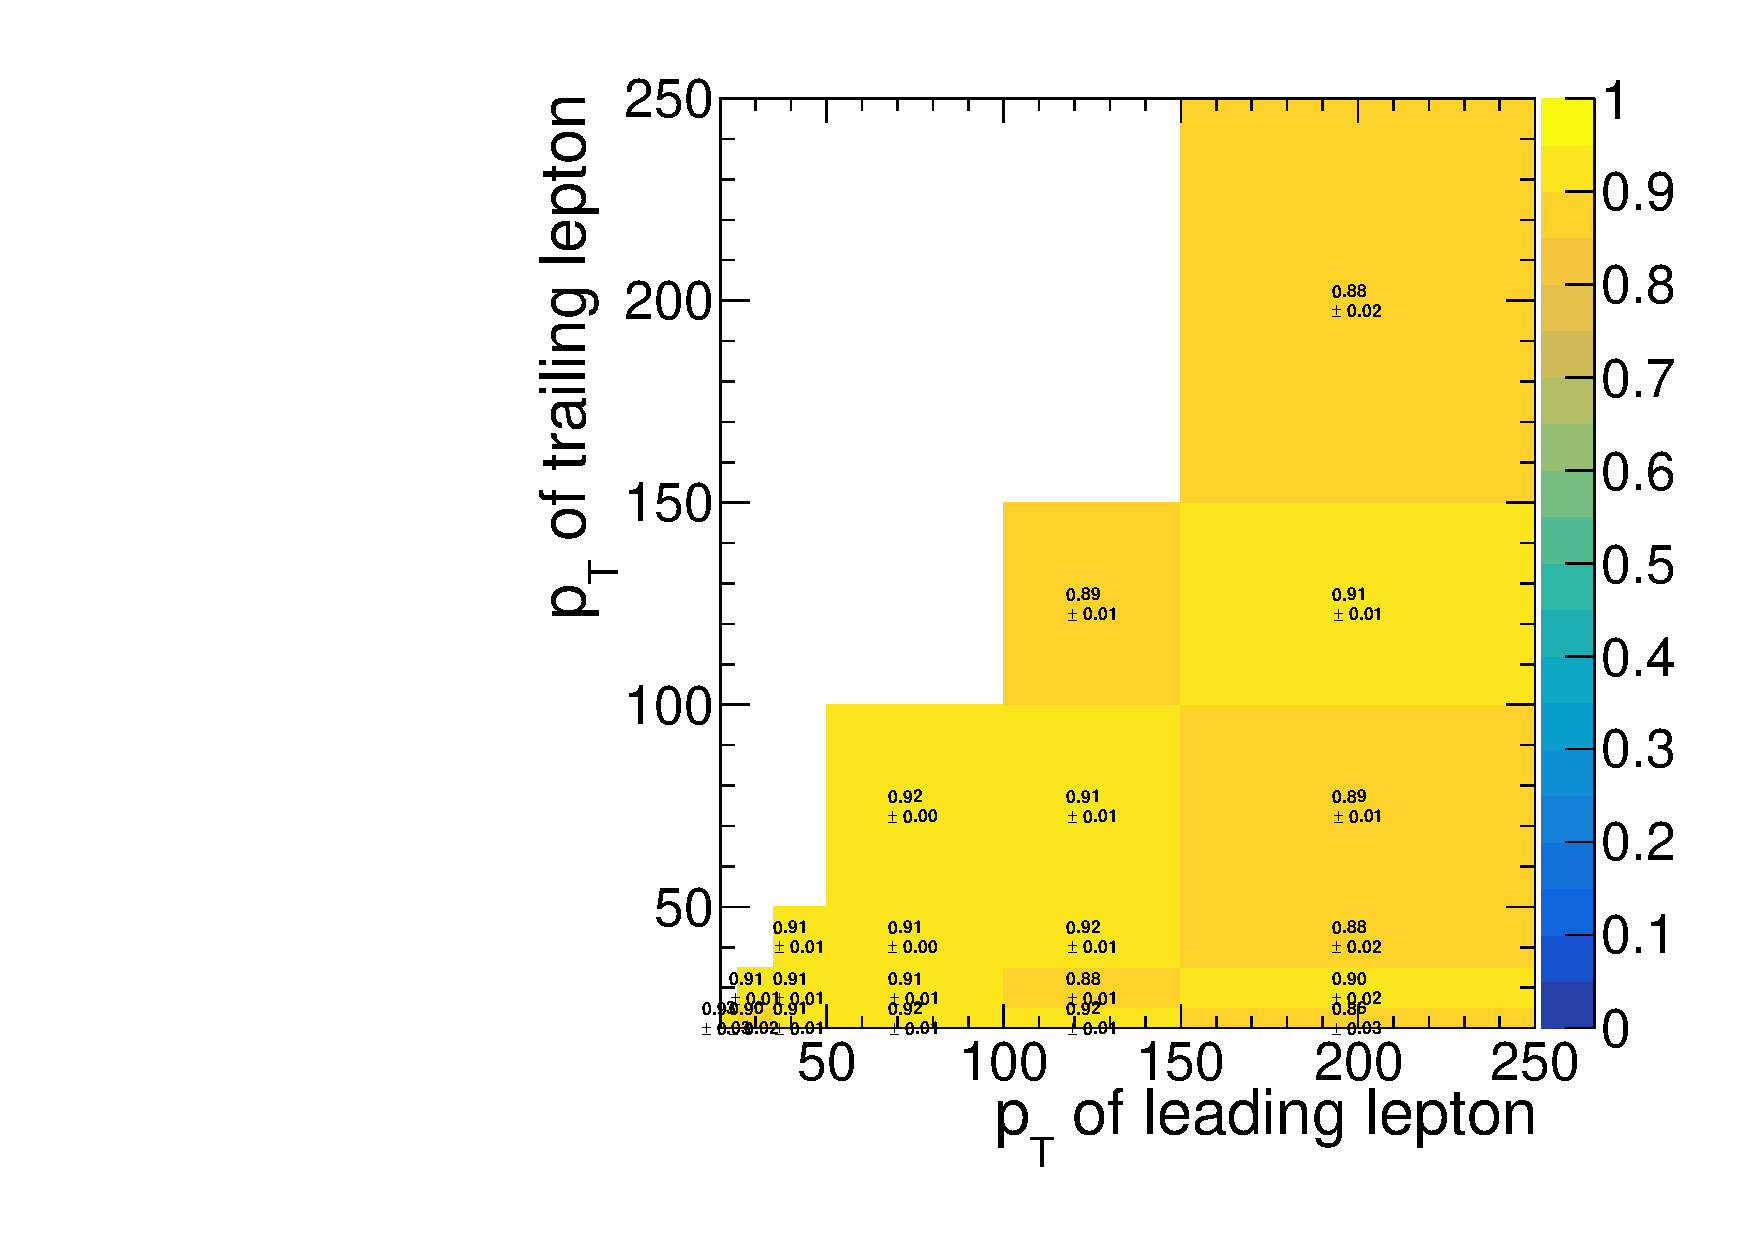
\includegraphics[width=0.45\textwidth]{figures/trigger/HLT_mue_pt1_pt2_lowEta1_veryCoarse.pdf}}
  \subfloat[][2l+backup, low $|\eta|$]  {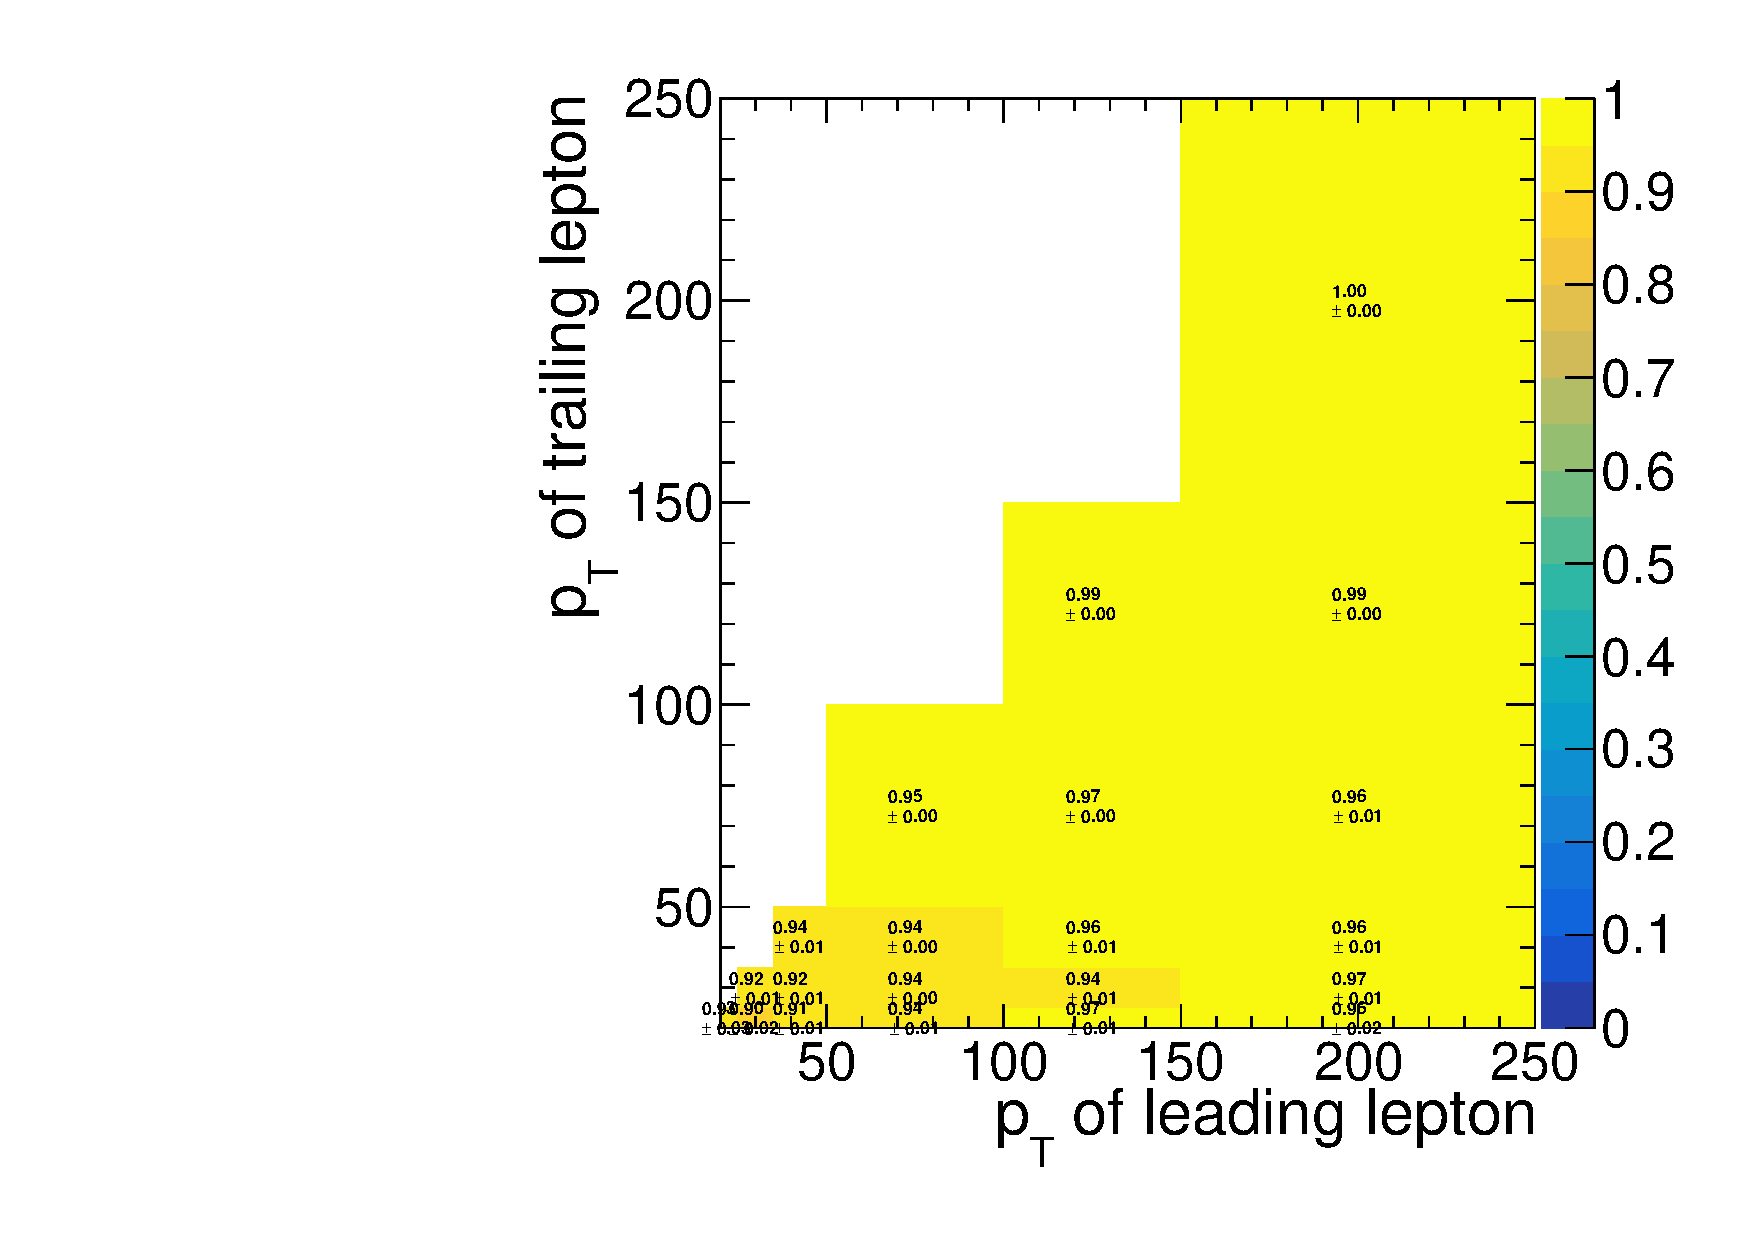
\includegraphics[width=0.45\textwidth]{figures/trigger/HLT_mue_OR_HLT_mu30e30_OR_HLT_SingleEle_noniso_OR_HLT_SingleMu_noniso_pt1_pt2_lowEta1_veryCoarse.pdf}}\\
  \subfloat[][only 2l, high $|\eta|$]   {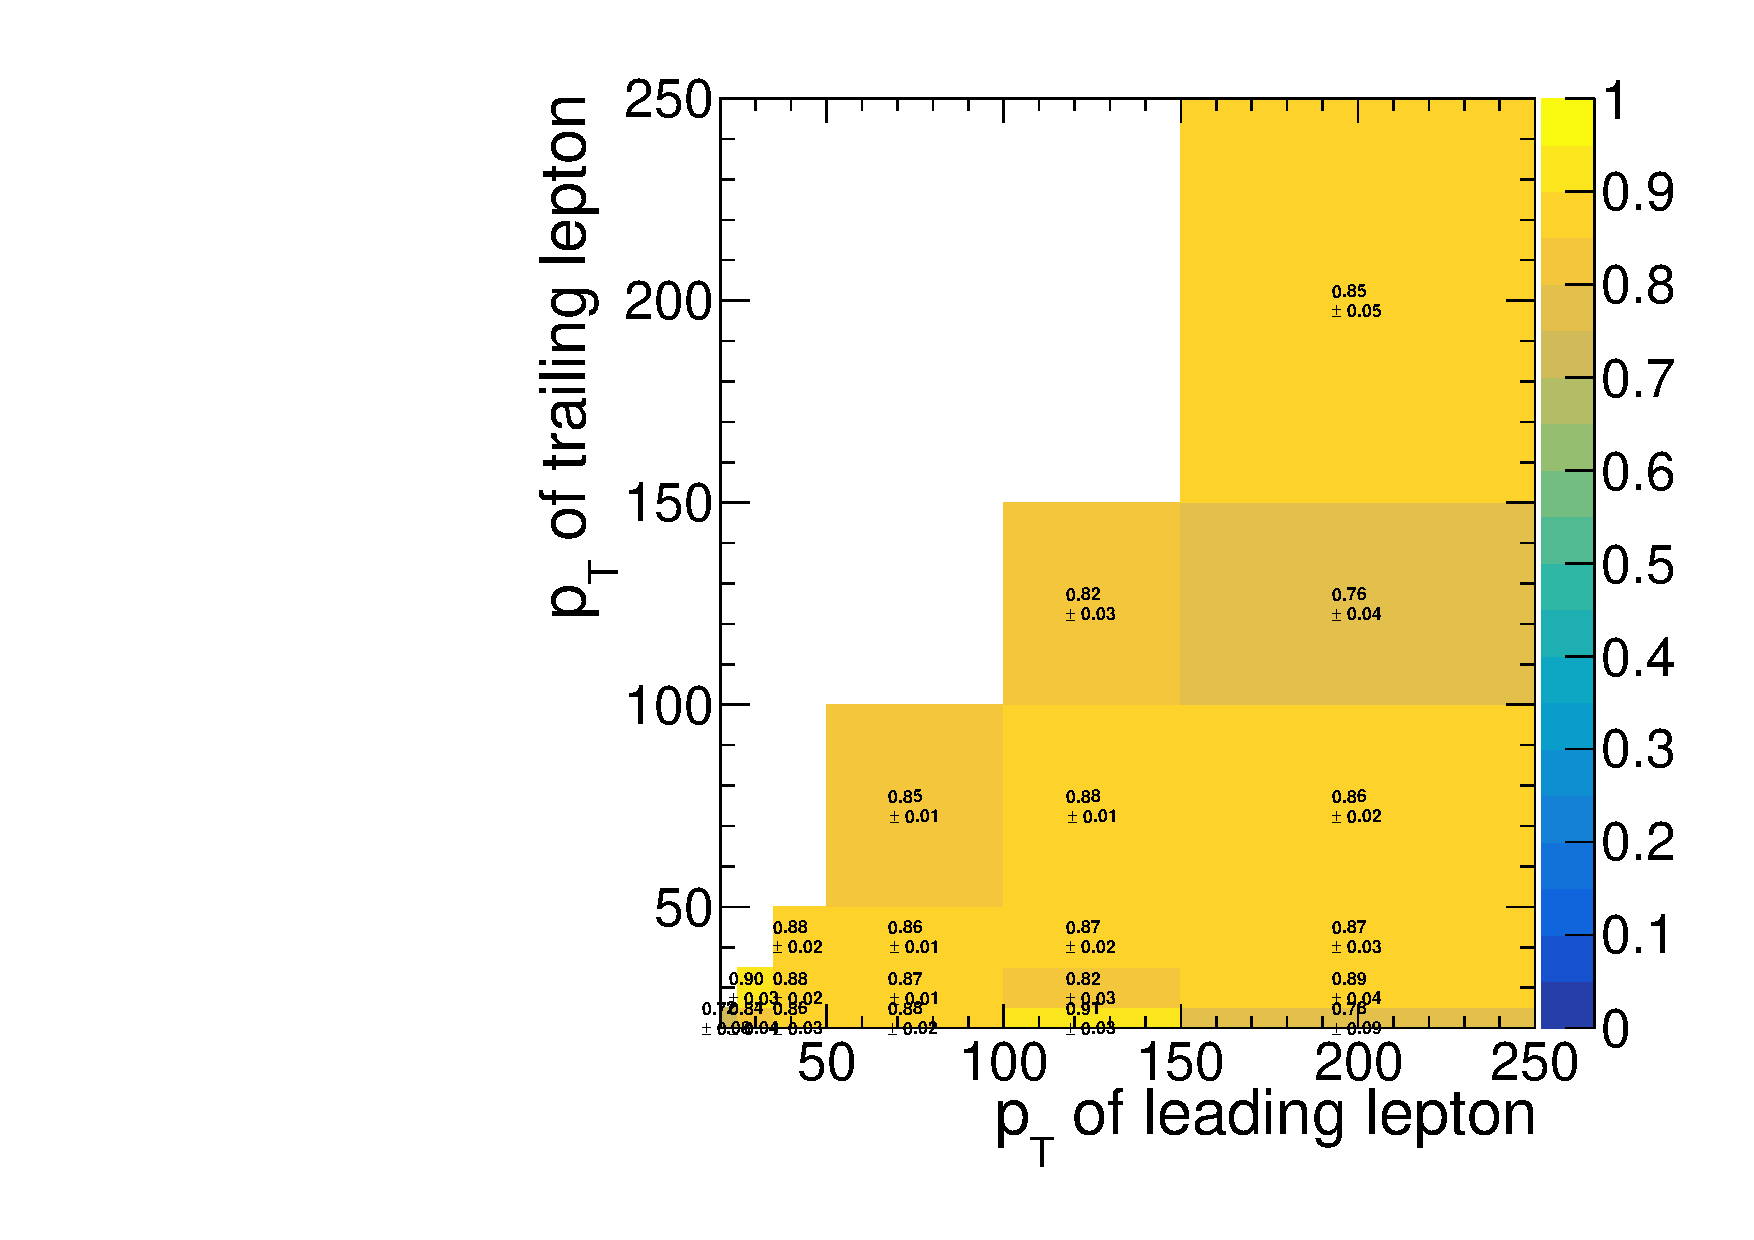
\includegraphics[width=0.45\textwidth]{figures/trigger/HLT_mue_pt1_pt2_highEta1_veryCoarse.pdf}}
  \subfloat[][2l+backup, high $|\eta|$] {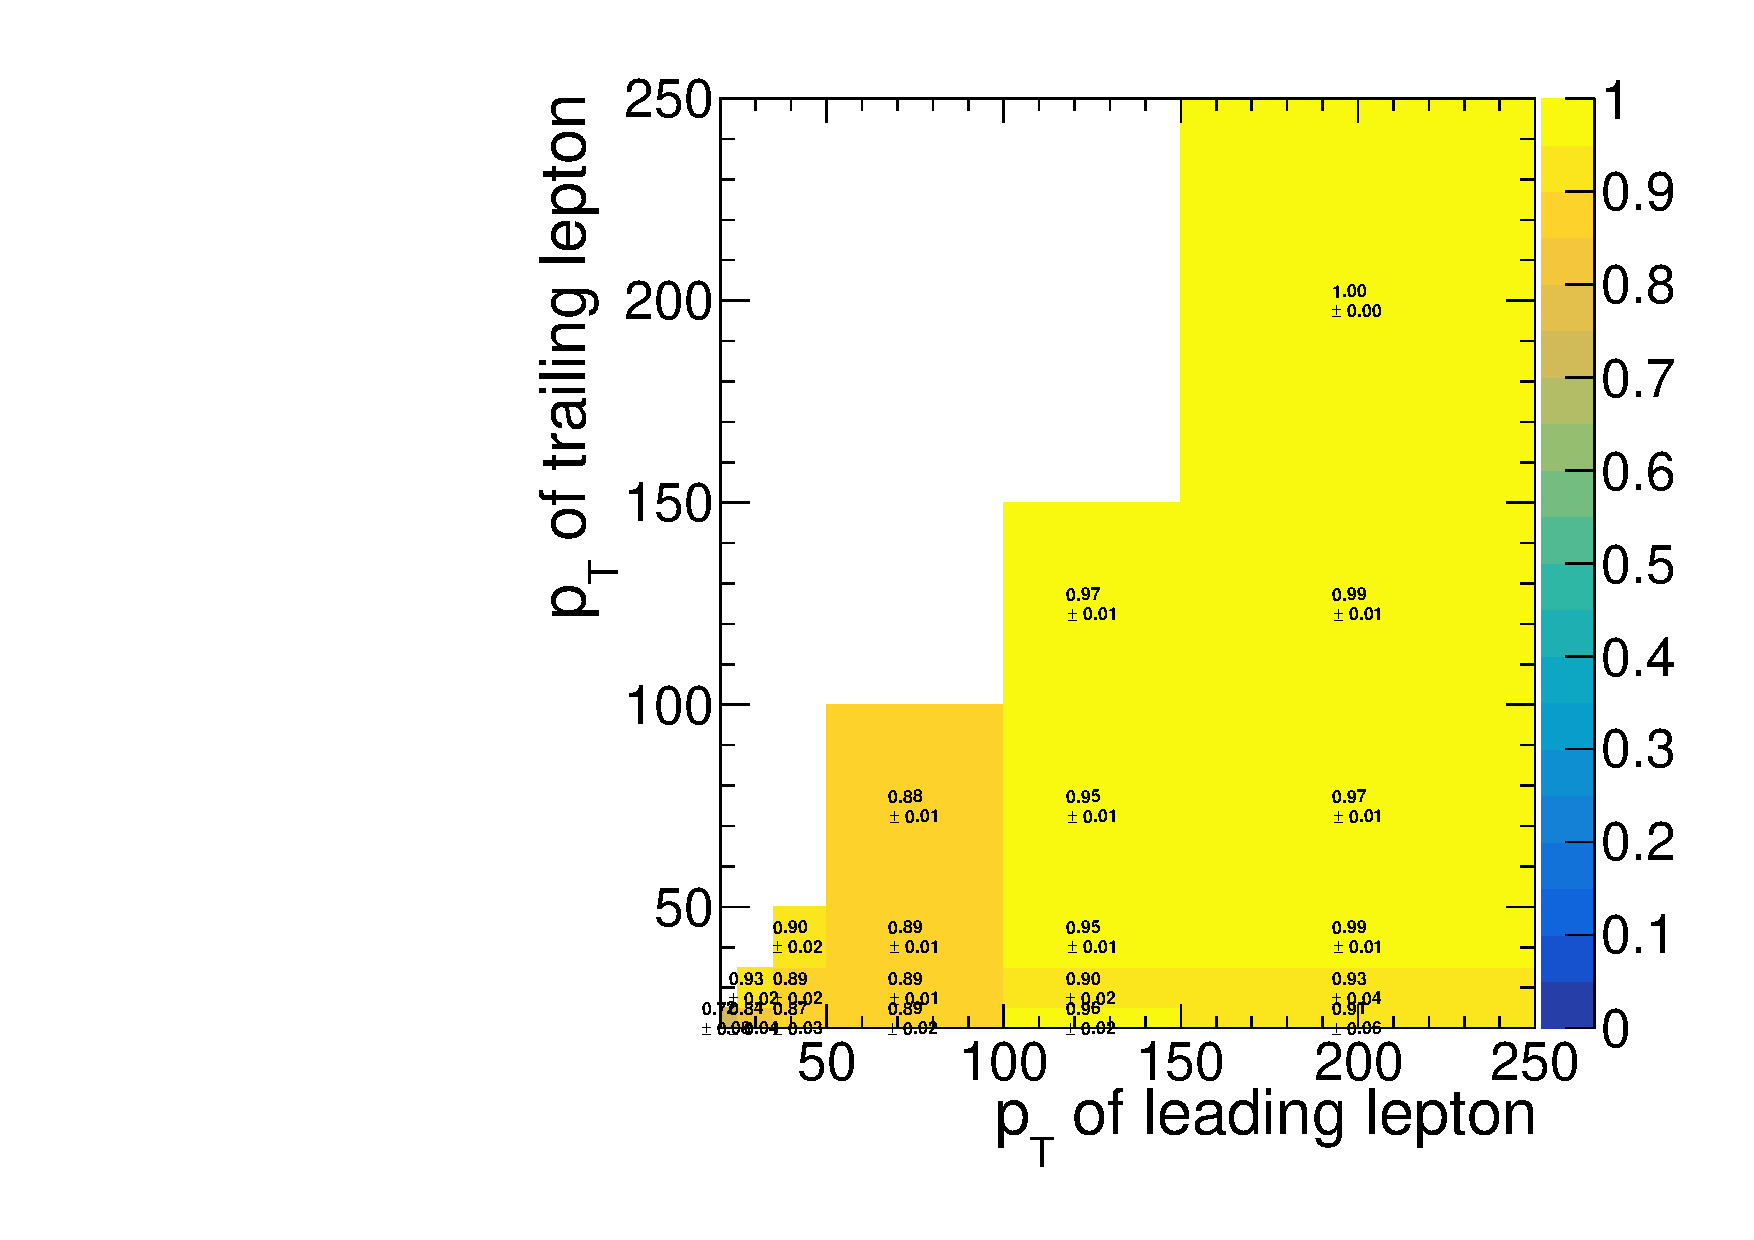
\includegraphics[width=0.45\textwidth]{figures/trigger/HLT_mue_OR_HLT_mu30e30_OR_HLT_SingleEle_noniso_OR_HLT_SingleMu_noniso_pt1_pt2_highEta1_veryCoarse.pdf}}
  \caption{Trigger efficiency maps for the e$\mu$ channel for $\eta$<1.5 (top) and $\eta>1.5$ (bottom) of the muon. The plots on the left show the efficiency of the  
double lepton triggers without the single lepton backup.}
  \label{fig:emu_triggerEff}
\end{figure}

\begin{figure}
  \centering
  \subfloat[][only 2l, low $|\eta|$]    {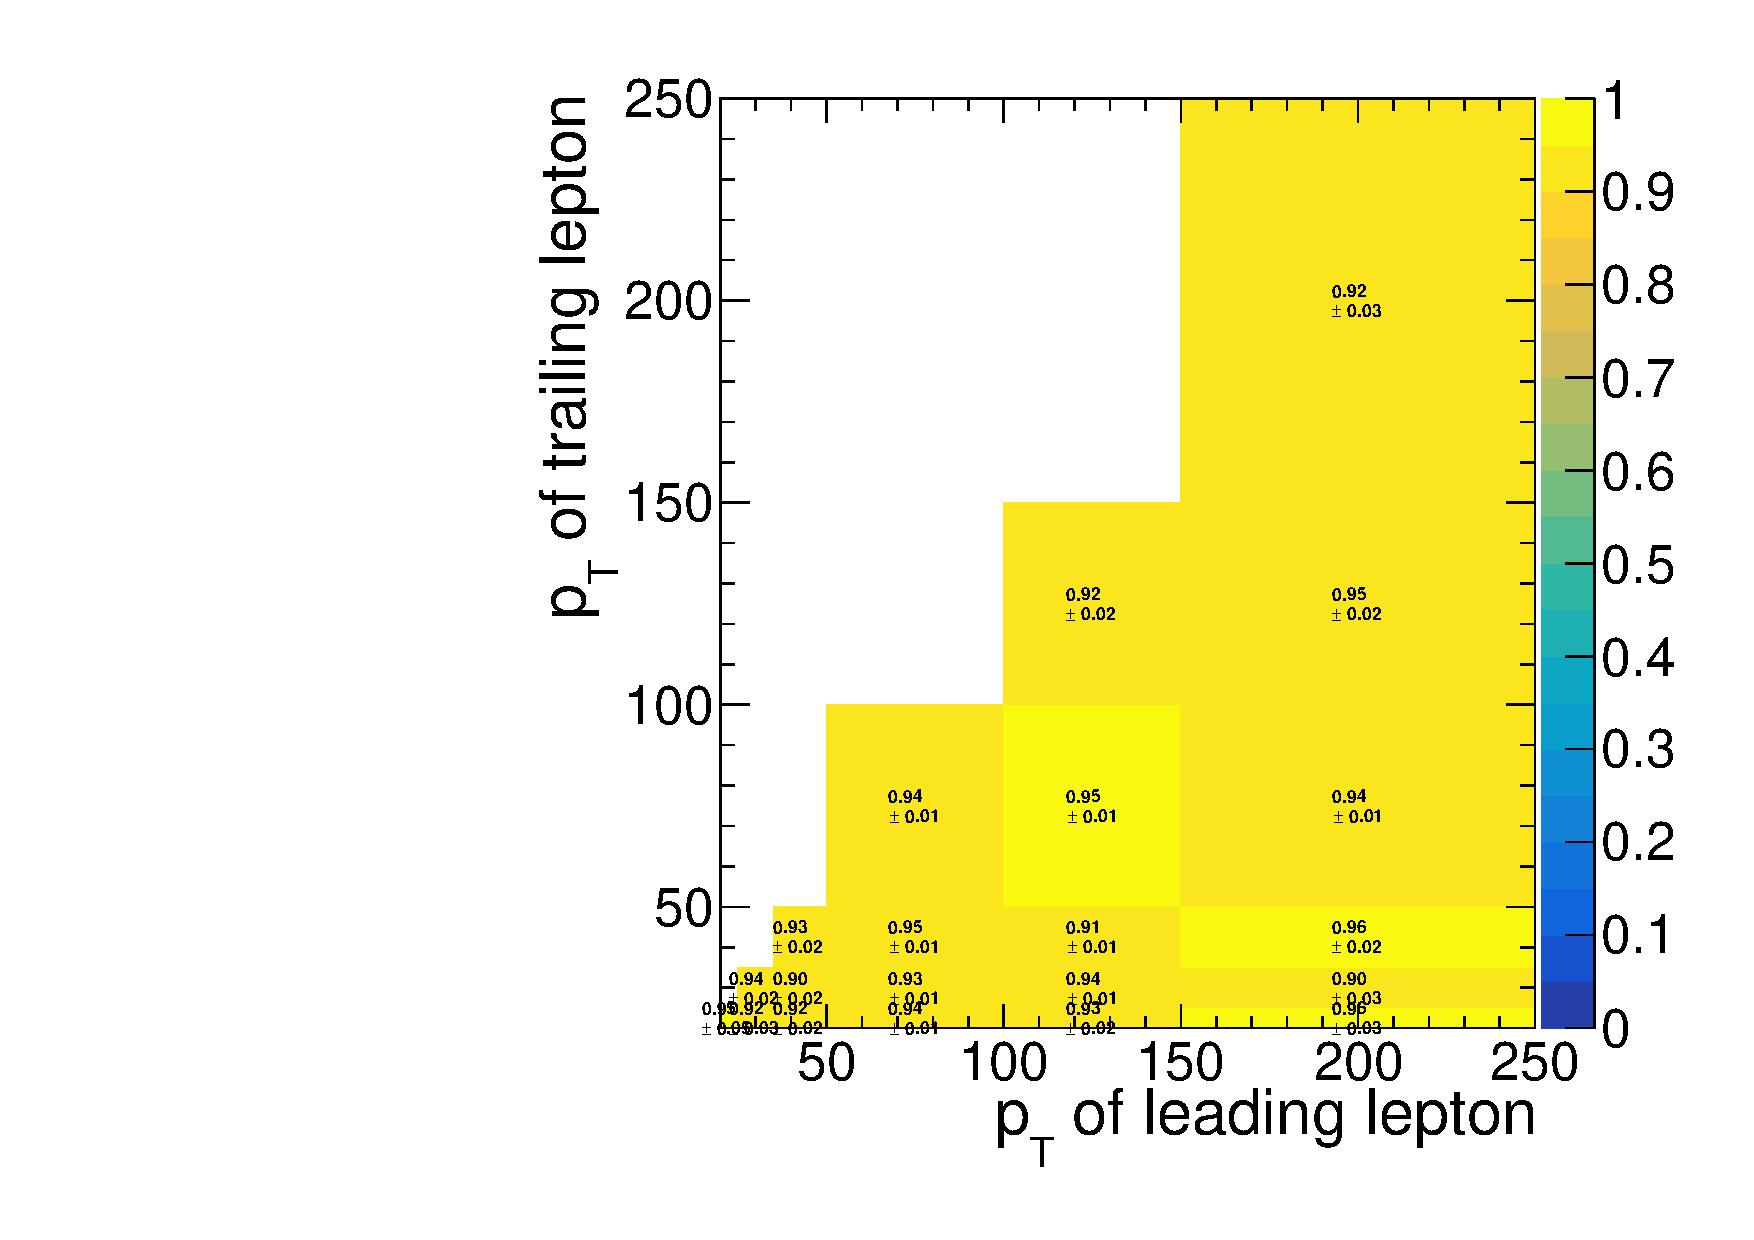
\includegraphics[width=0.45\textwidth]{figures/trigger/HLT_ee_DZ_pt1_pt2_lowEta1_veryCoarse.pdf}}
  \subfloat[][2l+backup, low $|\eta|$]  {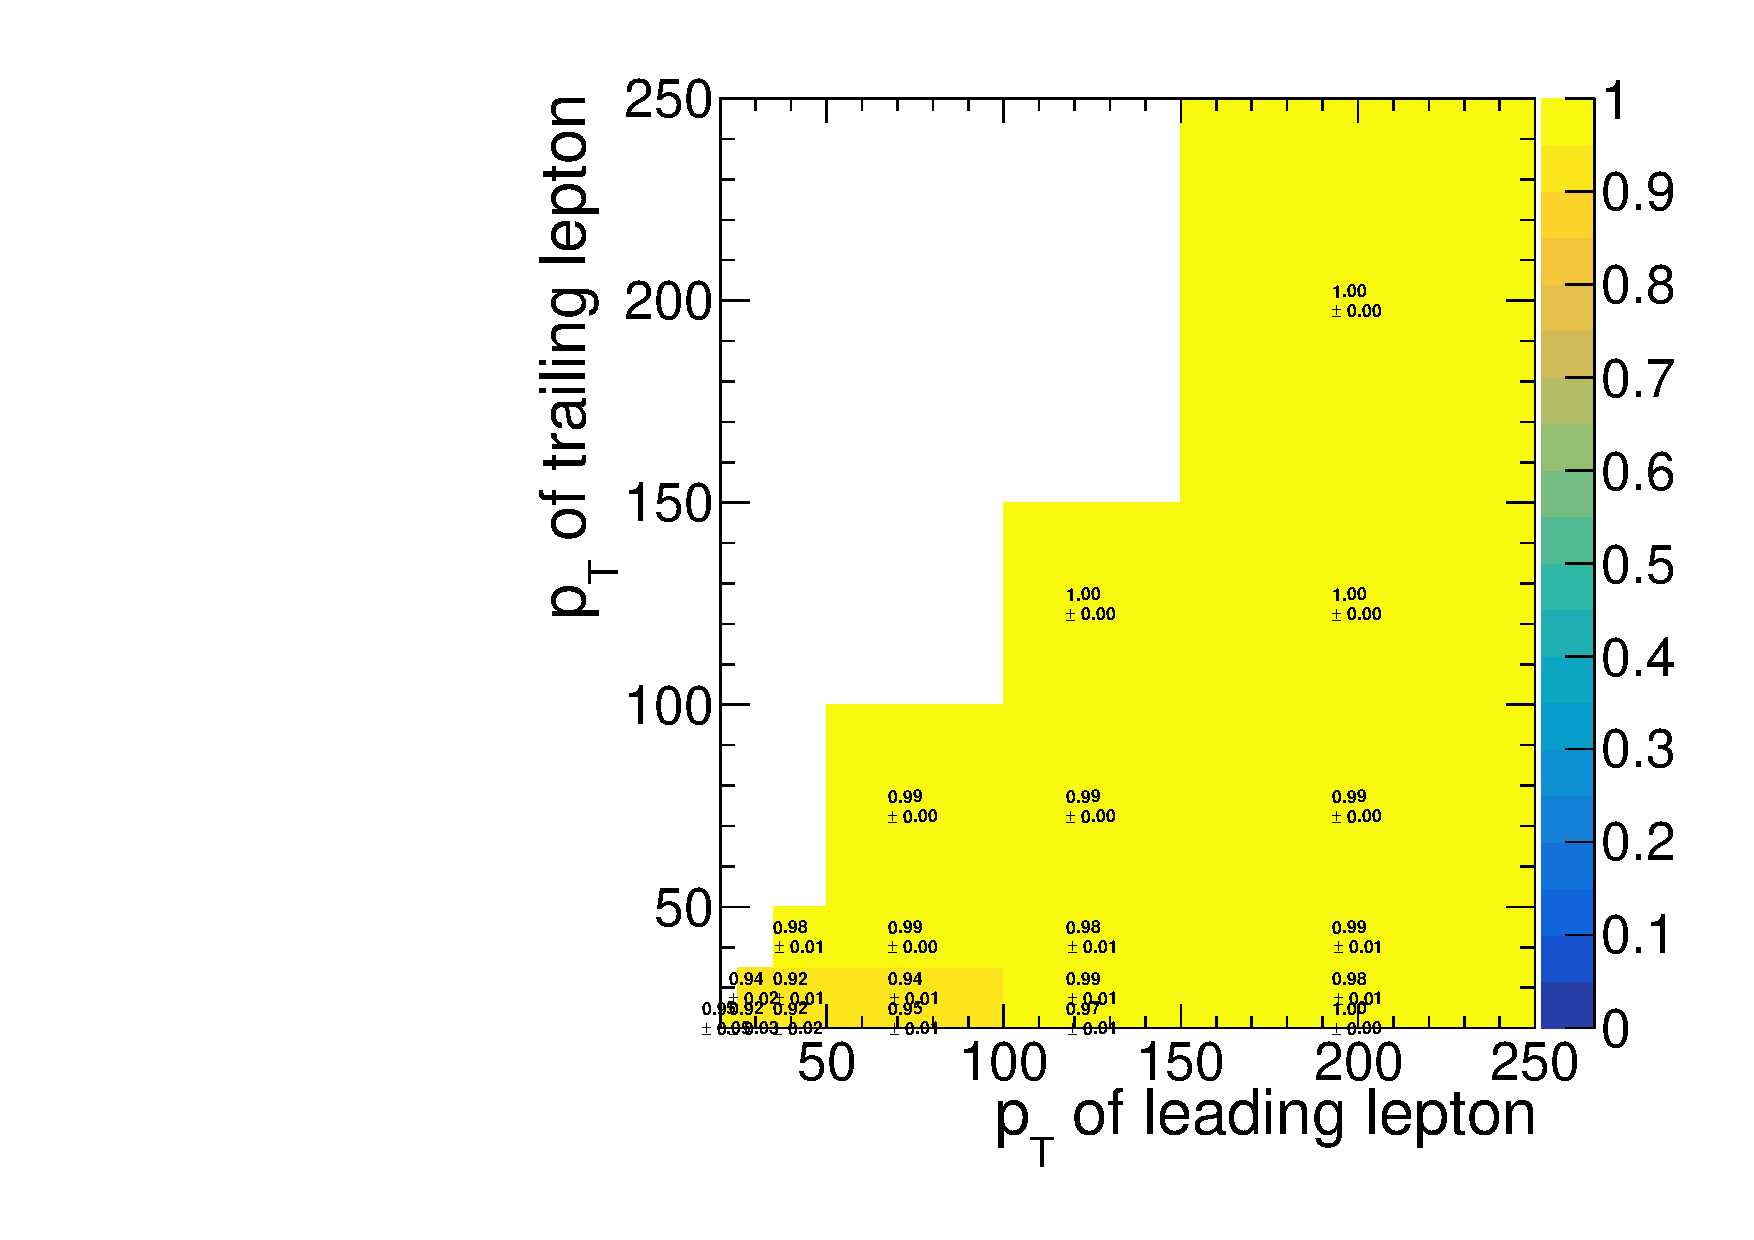
\includegraphics[width=0.45\textwidth]{figures/trigger/HLT_ee_DZ_OR_HLT_ee_33_OR_HLT_ee_33_MW_OR_HLT_SingleEle_noniso_pt1_pt2_lowEta1_veryCoarse.pdf}}\\
  \subfloat[][only 2l, high $|\eta|$]   {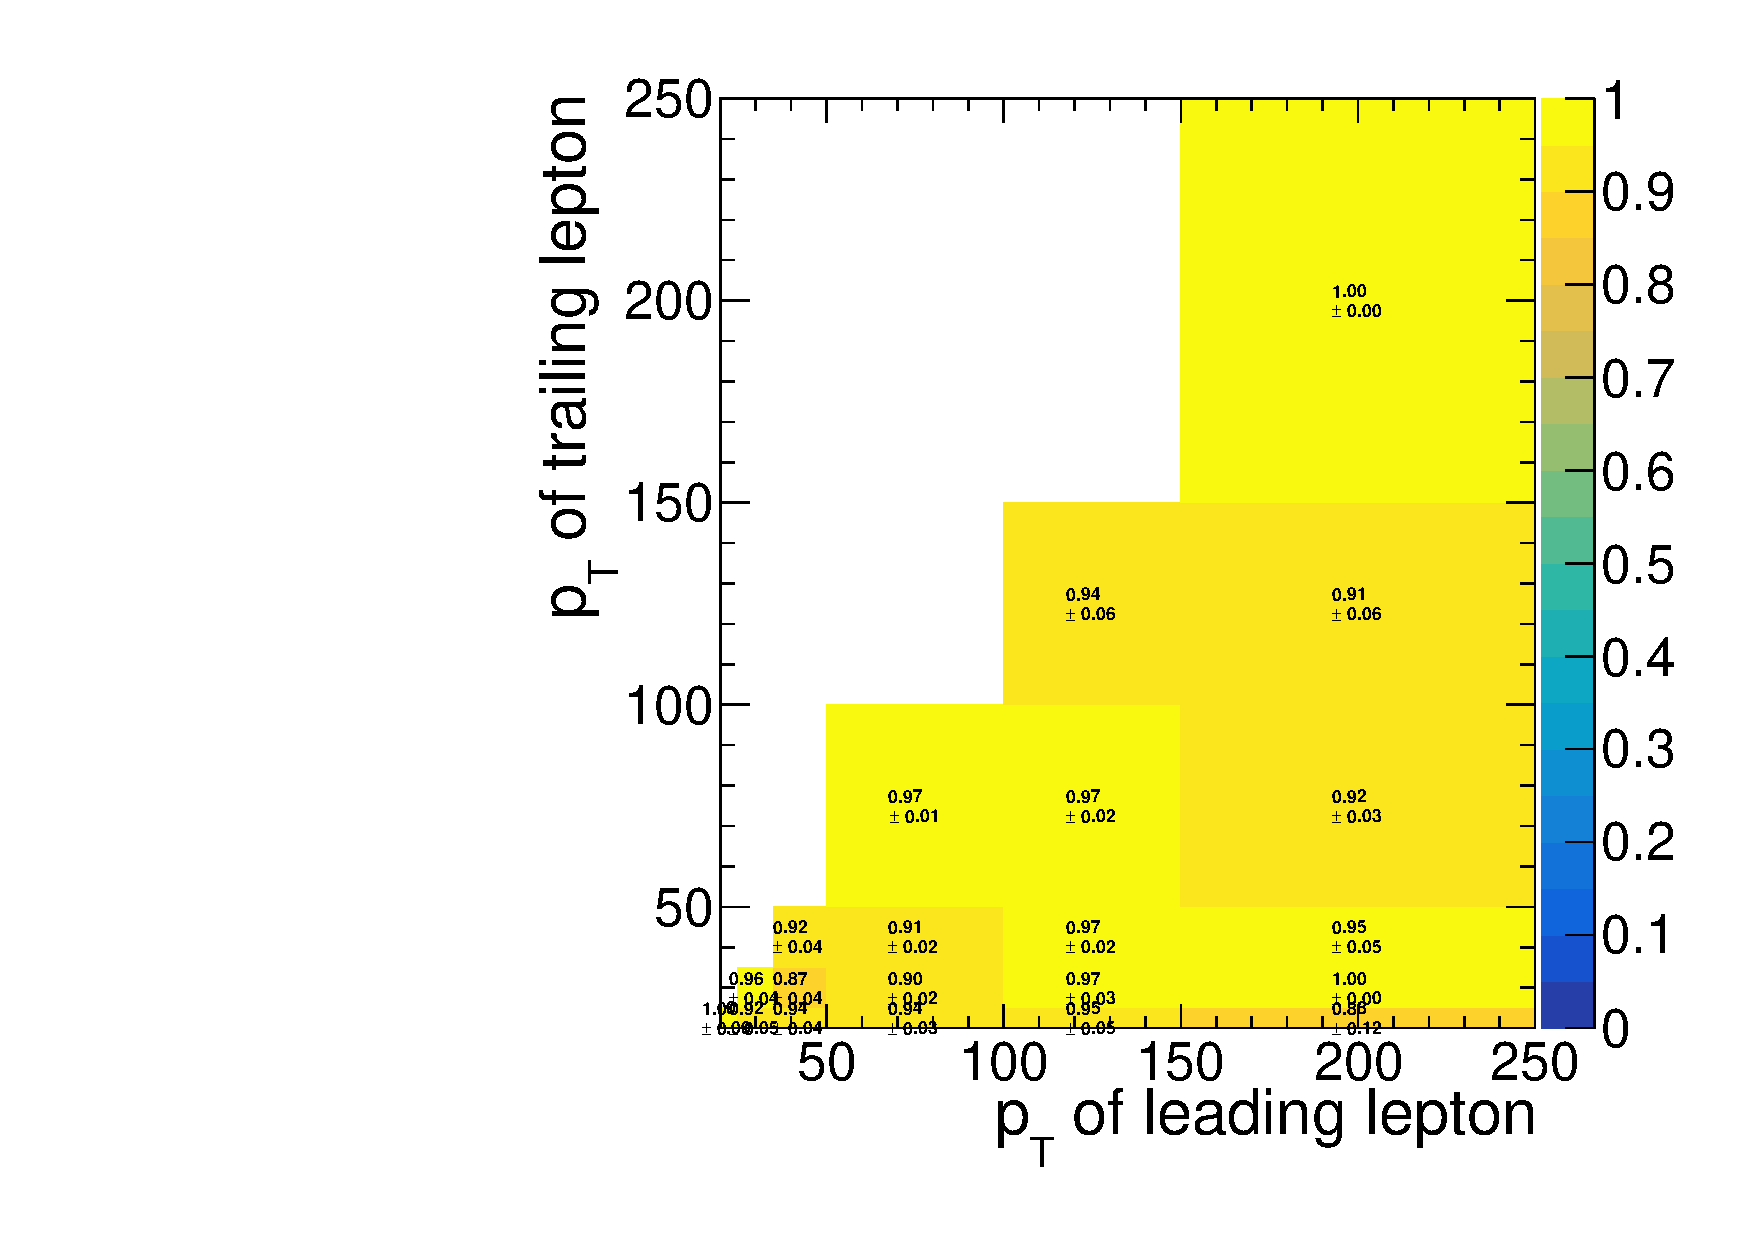
\includegraphics[width=0.45\textwidth]{figures/trigger/HLT_ee_DZ_pt1_pt2_highEta1_veryCoarse.pdf}}
  \subfloat[][2l+backup, high $|\eta|$] {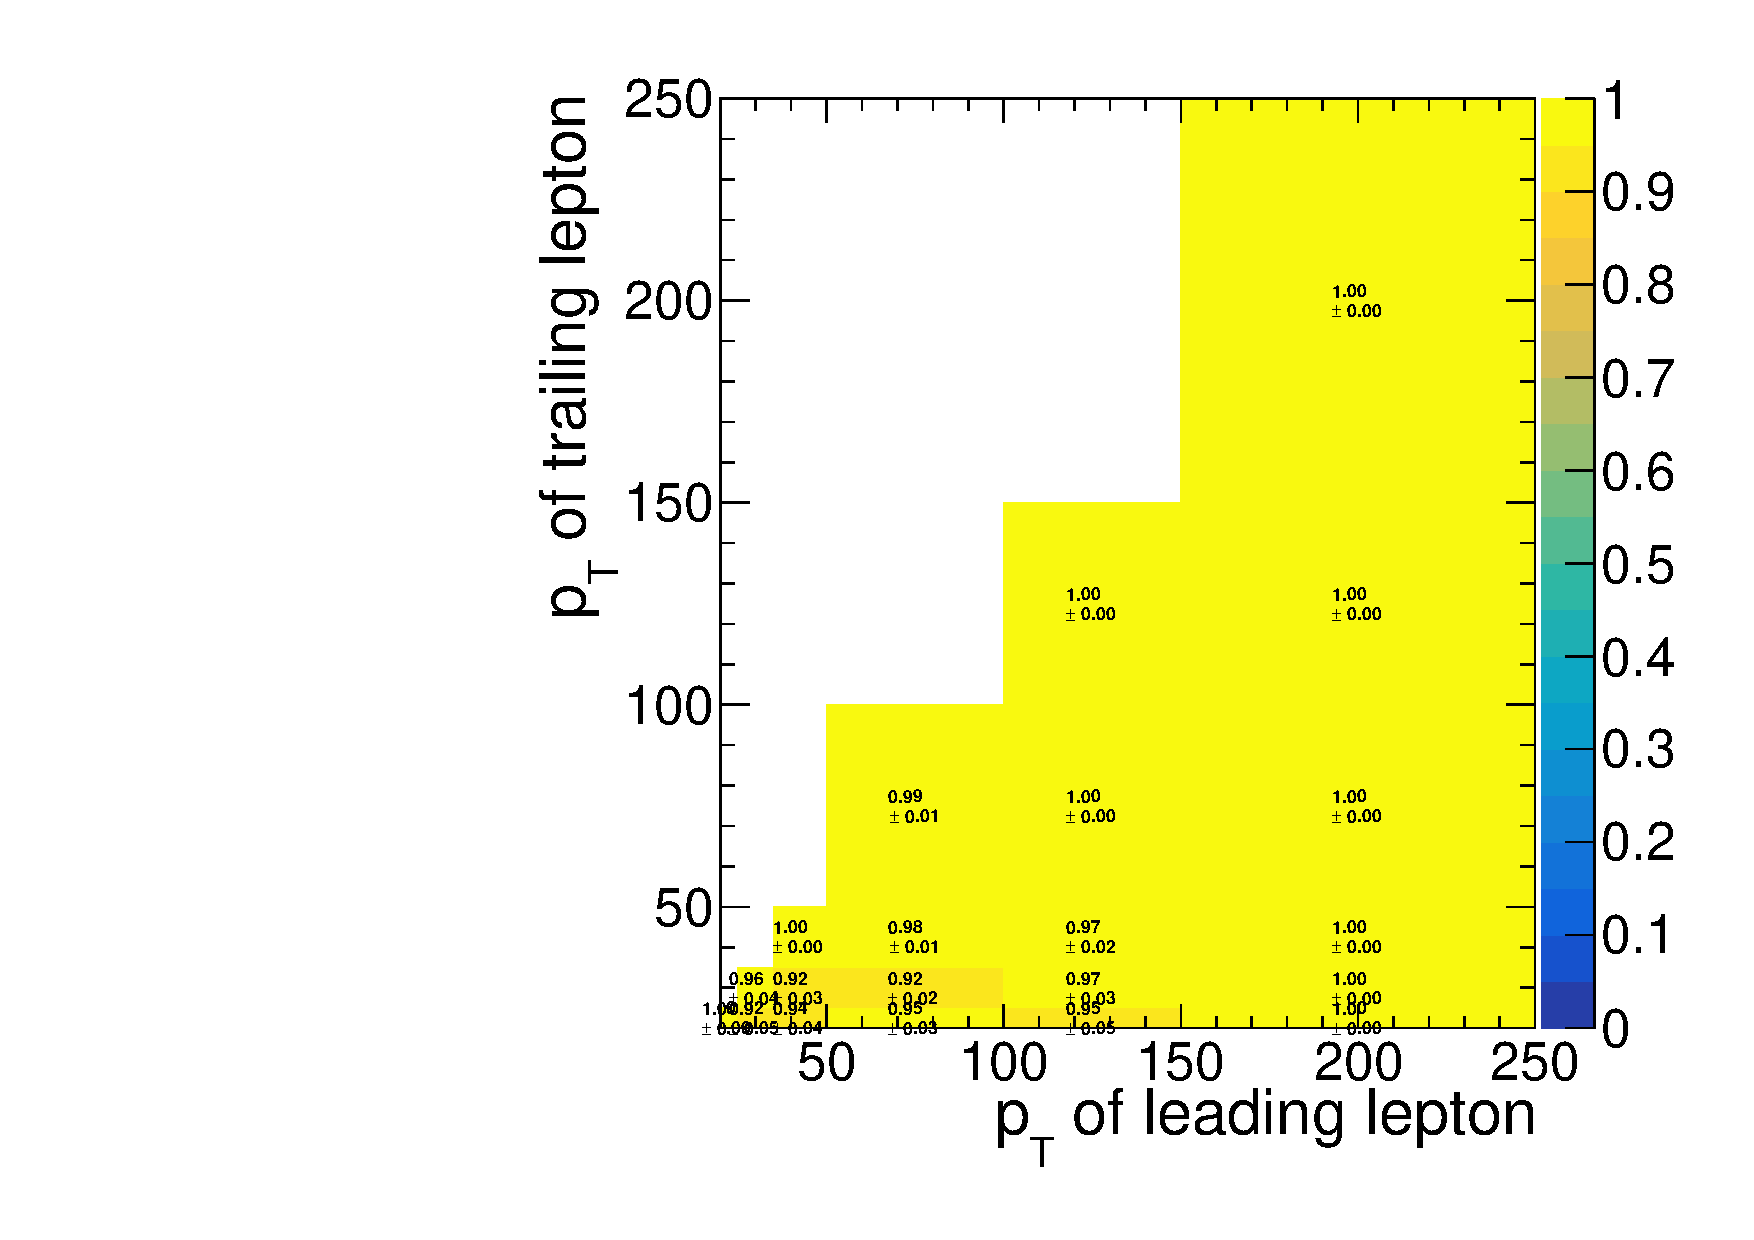
\includegraphics[width=0.45\textwidth]{figures/trigger/HLT_ee_DZ_OR_HLT_ee_33_OR_HLT_ee_33_MW_OR_HLT_SingleEle_noniso_pt1_pt2_highEta1_veryCoarse.pdf}}
  \caption{Trigger efficiency maps for the ee channel for $\eta$<1.5 (top) and $\eta>1.5$ (bottom) of the leading lepton. The plots on the left show the efficiency of the  
double lepton triggers without the single lepton backup. }
  \label{fig:ee_triggerEff}
\end{figure}


%{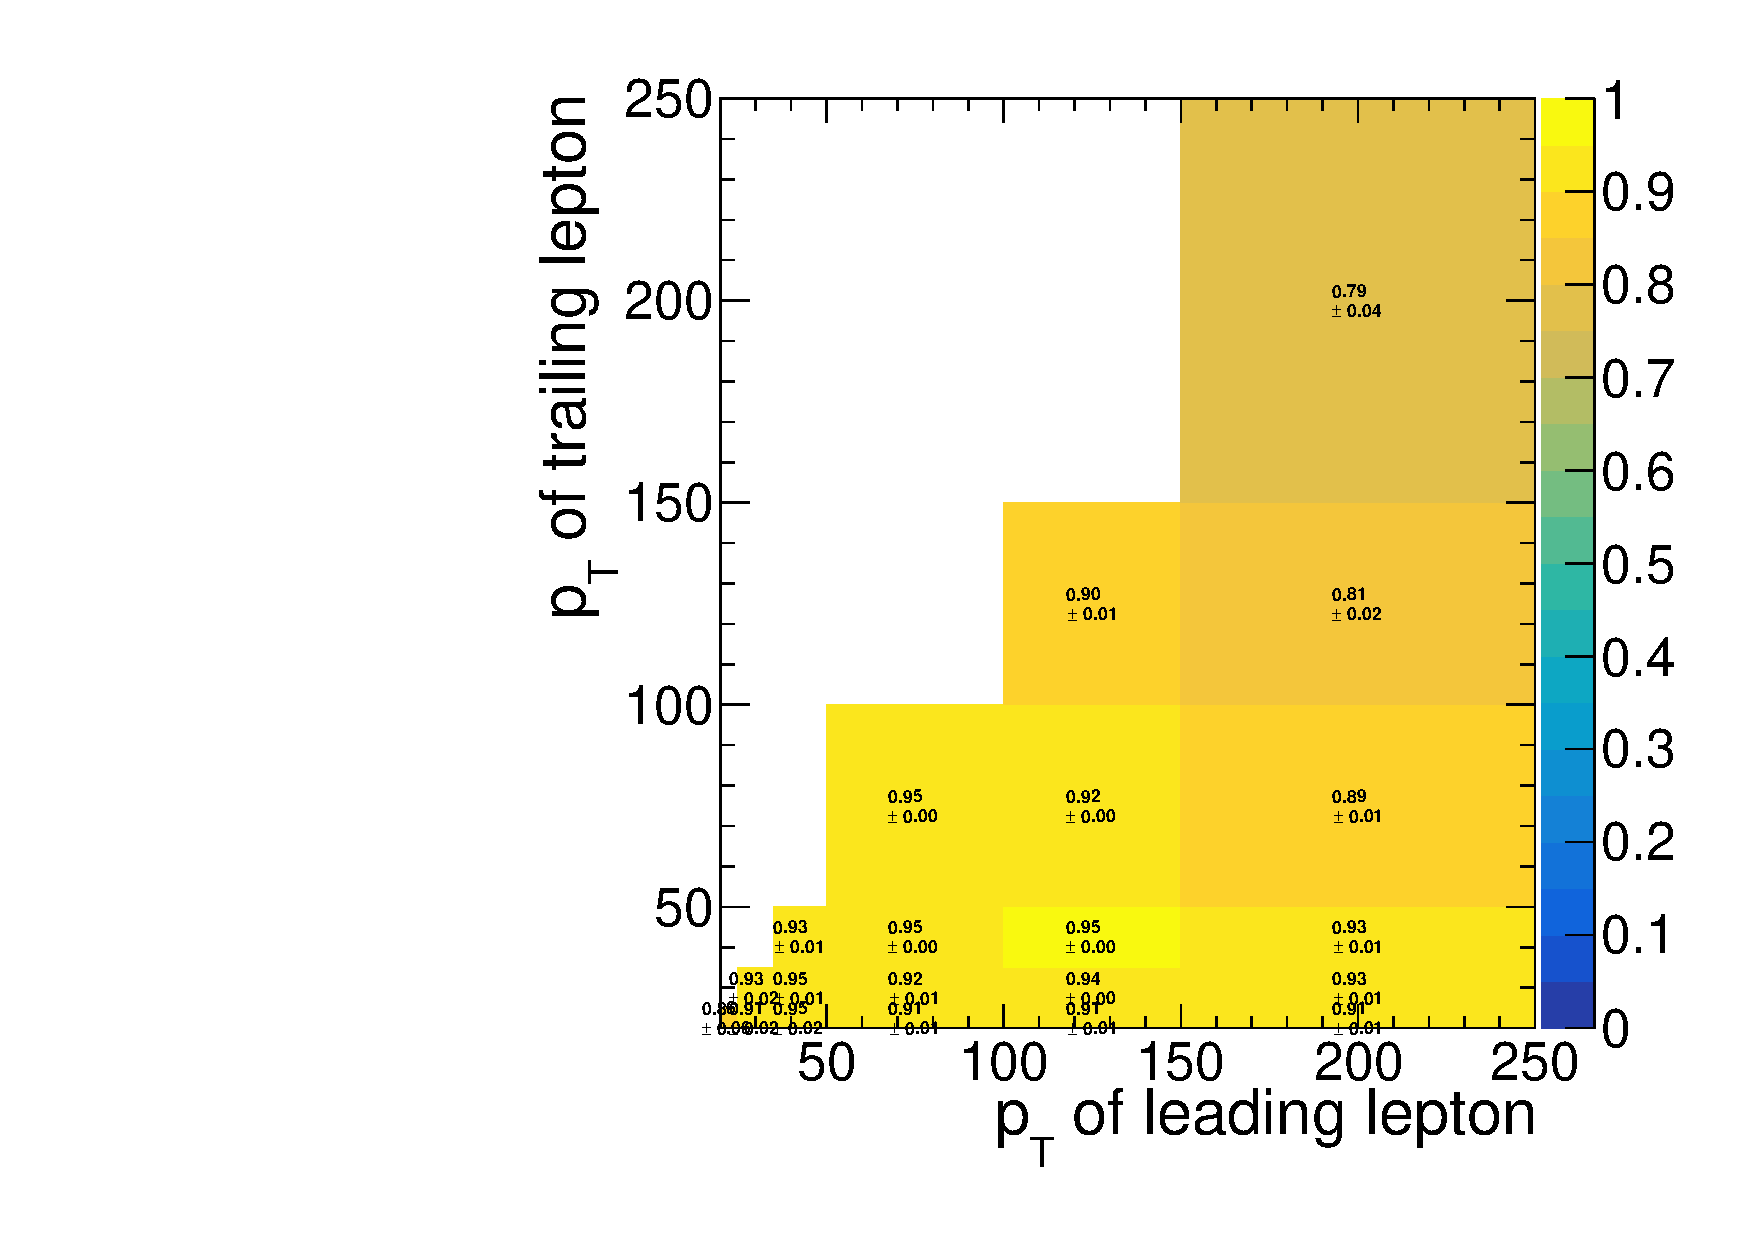
\includegraphics[width=0.5\textwidth]{figures/trigger/HLT_mumuIso_OR_HLT_mumuNoiso_pt1_pt2_highEta1_veryCoarse.pdf}}
%{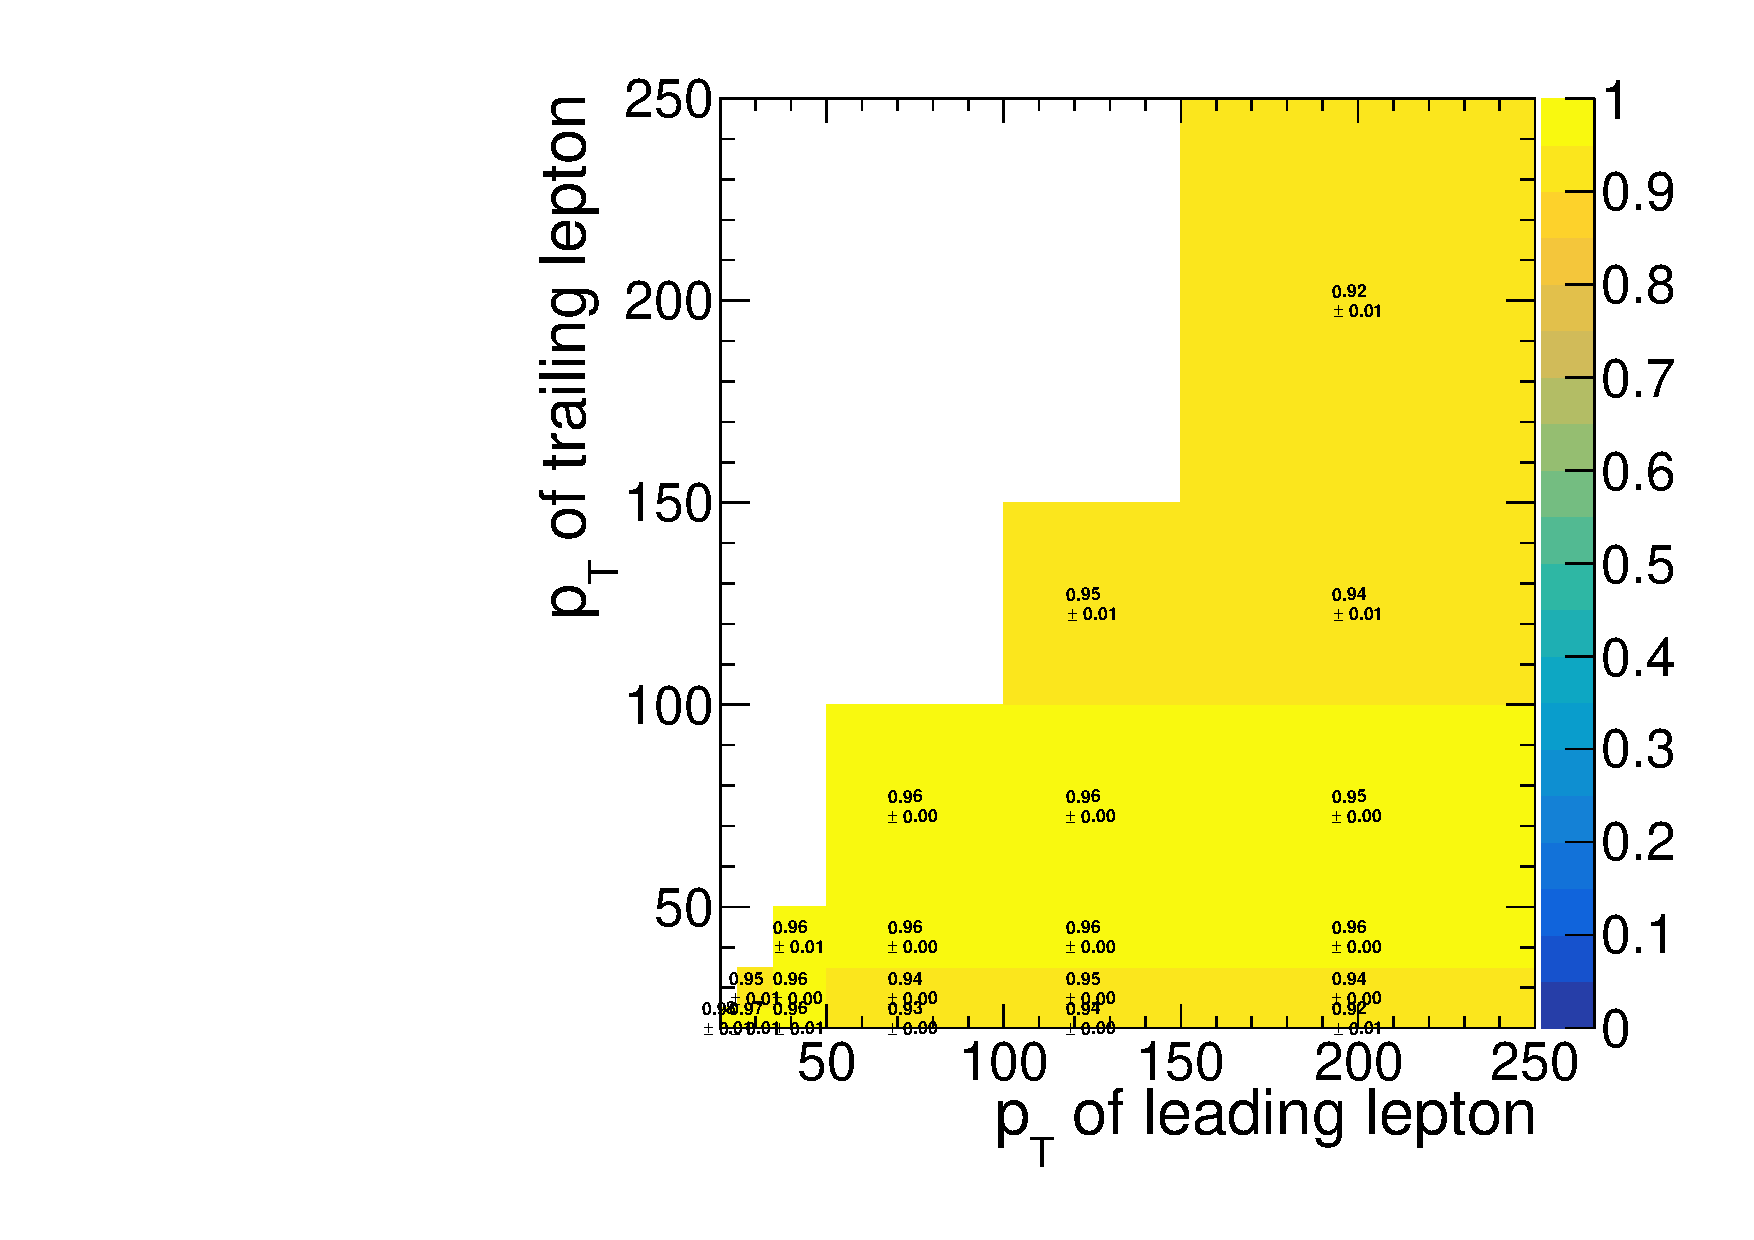
\includegraphics[width=0.5\textwidth]{figures/trigger/HLT_mumuIso_OR_HLT_mumuNoiso_pt1_pt2_lowEta1_veryCoarse.pdf}}

